\documentclass{article}
\usepackage[OT1]{fontenc}
\usepackage{graphicx}
\usepackage{setspace}
\usepackage{anysize}
\usepackage{enumerate}
\usepackage{amssymb}
\usepackage{algorithm2e}
\usepackage{amsthm}
\usepackage{amsmath}
\usepackage{booktabs}
\usepackage{ulem}
\marginsize{3cm}{3cm}{0cm}{3cm}

\fontfamily{ptm}\fontsize{14}{14}\selectfont 
\singlespacing
\newcommand{\solution}[1]{~\\ $\blacksquare$ \sffamily\upshape\selectfont #1
\normalfont ~\\~ }
\newcommand\independent{\protect\mathpalette{\protect\independenT}{\perp}}
\def\independenT#1#2{\mathrel{\rlap{$#1#2$}\mkern2mu{#1#2}}} 
\setlength{\parindent}{0pt}
% \setlength{\textwidth}{1.5\textwidth}

\begin{document}
\begin{center}
\textbf{\large{
HOMEWORK 3 \\
Introduction to Artifitial Intelligence \\}}
\textsc{\Large{Shumin Guo}}
\end{center}

\section{Execise 20.9}
Consider a single Boolean random variable $Y$ (the
"classification"). Let the prior probability P(Y = $true$) be $\pi$. Let's 
try to find $\pi$, given a training set $D=(y_1,\ldots,y_N)$ with N
independent samples of Y. Furthermore, suppose $p$ of the $N$ are positive
and $n$ of the $N$ are negative.
\begin{enumerate}[a.]
\item Write down an expression for the likelihood of D (i.e., the
probability of seeing this particular sequence of examples, given a
fixed value of $\pi$) in terms of $\pi$, and $n$.
\solution{
  $L(\pi) = \pi^n(1-\pi)^{N-n}$
}
\item By differentiating the log likelihood L, find the value of $\pi$
that maximizes the likelihood.
\solution{
  \begin{align*}
    \pi^{mle}&=\arg\max_{\pi}\pi^p(1-\pi)^n \\
    &= \arg\max_{\pi}plog\pi+nlog(1-\pi) \\
    &= \pi ~s.t.~ \frac{\partial LL}{\partial \pi} = 0 \\ 
    &= \pi ~s.t.~ p\frac{1}{\pi}+n\frac{1}{1-\pi} = 0 \\
    &= \frac{p}{n+p}
  \end{align*}
}
\item Now suppose we add in $k$ Boolean random variables $X_1, X_2,\ldots,X_k
$ (the "attributes") that describe each sample. and suppose we assume
that the attributes are conditionally independent of each other given
the goal Y. Draw the Bayes net corresponding to this assumption.
\solution{
See Bayesian network in Figure \ref{fig:20_1c}.
  \begin{figure}[ht]
    \centering
    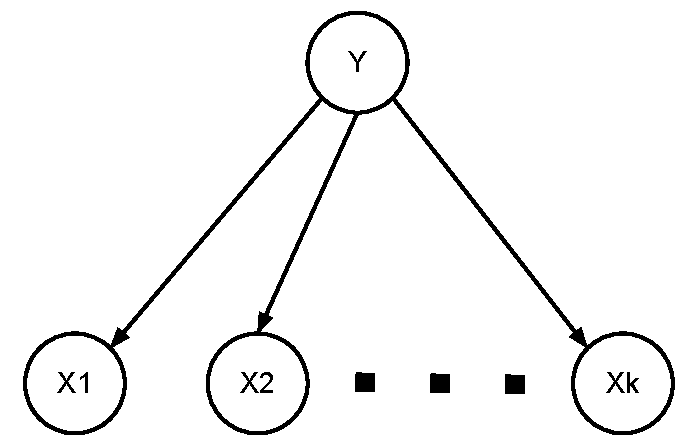
\includegraphics[width=.5\textwidth]{AI-HWK3_1c.pdf}
    \caption{Bayesian Network for question c.}\label{fig:20_1c}
  \end{figure}
}
\item Write down the likelihood for the data including the attributes,
using the following additional notation:
\begin{itemize}
\item $\alpha_i$ is $P(X_i=true|Y=true)$.
\item $\beta_i$ is $P(X_i = true|Y = false)$.
\item $p_i^+$ is the count of samples for which $X_i = true$ and $Y = true$.
\item $n_i^+$ is the count of samples for which $X_i = false$ and $Y = true$.
\item $p_i^-$ is the count of samples for which $X_i = true$ and $Y = false$.
\item $n_i^-$ is the count of samples for which $X_i = false$ and $Y = false$.
\end{itemize}

[Hint: consider first the probability of seeing a single example with
specified values for $X_1, X_2,\ldots,X_k$ and $Y$.]
\solution{
  We use Y to denote $Y=true$ $\neg Y$ to denote $Y=false$, $X_i$ to denote
  $X_i=true$ and $\neg X_i$ to denote $X_i=false$. 
  \begin{align*}
    & P(x_{11},\ldots,x_{1k},\ldots,x_{N1},\ldots,x_{Nk},y_1,\ldots,y_N) \\
    & = \prod_{i=1}^N\prod_{j=1}^kP(x_{ij}|y_i)P(y_i) \\
    & = (\prod_{i=1}^NP(y_i))(\prod_{j=1}^k(\prod_{i=1}^pP(x_{ij}|y_i))(\prod_{i=1}^nP(x_{ij}|y_i))) \\
    & = \pi^p(1-\pi)^n(\prod_{j=1}^k(\prod_{i=1}^{p_j^+}P(x_{ij}|y_i))(\prod_{i=1}^{n_j^+}P(x_{ij}|y_i)) 
    (\prod_{i=1}^{p_j^-}P(x_{ij}|y_i))(\prod_{i=1}^{n_j^-}P(x_{ij}|y_i)) \\
    & = \pi^p(1-\pi)^n(\prod_{j=1}^k(\prod_{i=1}^{p_j^+}P(X_j|Y))(\prod_{i=1}^{n_j^+}P(\neg X_j|Y)) 
    (\prod_{i=1}^{p_j^-}P(X_j|\neg Y))(\prod_{i=1}^{n_j^-}P(\neg X_j|\neg Y)) \\
    & = \pi^p(1-\pi)^n\prod_{j=1}^k\alpha_j^{p_j^+}(1-\alpha_j)^{n_j^+}\beta_j^{p_j^-}(1-\beta_j)^{n_j^-} \\
    &\mbox{\rmfamily\selectfont{By replacing j to i.}\normalfont} \\
    & = \pi^p(1-\pi)^n\prod_{i=1}^k\alpha_i^{p_i^+}(1-\alpha_i)^{n_i^+}\beta_i^{p_i^-}(1-\beta_i)^{n_i^-} 
  \end{align*}
}

\item By differentiating the log likelihood L, find the values of
  $\alpha_i$ and $\beta_i$ (in terms of the various counts) that
  maximize the likelihood and say in words what these values represent.
\solution{
  \begin{align*}
    LL & = plog\pi + nlog(1-\pi) + \sum_{i=1}^k(p_i^+log\alpha_i + n_i^+log(1-\alpha_i) 
    + p_i^-log\beta_i + n_i^-log(1 - \beta_i)) \\ 
    \frac{\partial(LL)}{\partial\alpha_i} & = \sum_{i=1}^k(\frac{p_i^+}{\alpha_i} 
    - \frac{n_i^+}{1-\alpha_i}) = 0  \\
    &\Rightarrow \alpha_i=\frac{p_i^+}{p_i^++n_i^+} \\
    \frac{\partial(LL)}{\partial\beta_i} &= \sum_{i=1}^k(\frac{p_i^-}{\beta_i} 
    - \frac{n_i^-}{1-\beta_i}) = 0  \\
    &\Rightarrow \beta_i = \frac{p_i^-}{p_i^-+n_i^-}
  \end{align*}
  Explanations: $\alpha_i$ is the ratio of $X_i=true$ when $Y=true$ and Similarly, 
  $\beta_i$ is the ratio of $X_i=true$ when $Y=false$. 
}
\item Let $k = 2$, and consider a data set with 4 all four possible
examples of the \textsc{Xor} function. Compute the maximum likelihood
estimates of $\pi, \alpha_1, \alpha_2, \beta_1$ and $\beta_2$.
\solution{
  Samples can be found in Table \ref{tbl:1-f}. 
  \begin{table}[h]
    \centering
    \begin{tabular}{ccc}
      \toprule
      \textbf{$X_1$} & \textbf{$X_2$} & \textbf{$Y$} \\ \toprule
      0 & 0 & 0 \\ \midrule
      0 & 1 & 1 \\ \midrule
      1 & 0 & 1 \\ \midrule
      1 & 1 & 0 \\ \bottomrule
    \end{tabular}
    \caption{Sample data using XOR function.}
    \label{tbl:1-f}
  \end{table}

  According to the sample data, we can get the counts as follows: 
  \[p_1^+=1, p_2^+=1, n_1^+=1, n_2^+=1, p_1^-=1, p_2^-=1, n_1^-=1, n_2^-=1\].
  And the maximum likelihood values are: \[\pi = 0.5, \alpha_1 = 0.5, 
  \alpha_2 = 0.5, \beta_1 = 0.5, \beta_2 = 0.5.\]
}
\item Given these estimates of $\pi, \alpha_1, \alpha_2, \beta_1$ and
  $\beta_2$, what are the posterior probabilities $P(Y = true|x_1,x_2)$
  for each example? 
\solution{
  \begin{align*}
    P(Y|x_1,x_2) & = \frac{P(x_1,x_2|Y)P(Y)}{P(x_1,x_2)} \\ 
    & = \frac{P(x_1|Y)P(x_2|Y)P(Y)}{P(x_1)P(x_2)} ~ where ~ P(x_1=1) = P(x_2=1) = 0.5\\ 
    & = \frac{0.5\times 0.5\times 0.5}{0.5\times 0.5} \\ 
    & = 0.5 
  \end{align*}
  The posterior probability $P(Y=true|x_1,x_2) = 0.5$ for all the examples.
}
\end{enumerate}

\section{Execise 2.}
\[ p(x|\mu_1,\mu_2)=\frac{1}{3}\sqrt{2\pi}exp(-\frac{1}{2}(x-\mu_1)^2) +
\frac{2}{3\sqrt{2\pi}}exp(-\frac{1}{2}(x-\mu_2)^2) \]
The 25 samples (0.608,-1.590, 0.235, 3.949,-2.249, 2.704,-2.473,
0.672, 0.262, 1.072,-1.773, 0.537, 3.240, 2.400,-2.499, 2.608,-3.458,
0.257, 2.569, 1.415, 1.410,-2.653, 1.396, 3.286,-0.712) were drawn
from this mixture with mean $\mu_1$ = -2 and $\mu_2$ = 2. Using these
25 samples to estimate $\mu_1$ and $\mu_2$ by maximum likelihood
principle through EM algorithm with initial values (a)
$\hat{\mu}^{(0)} = 1$ and $\hat{\mu}^{(2)=3}$; $(b)\hat{\mu}^{(0)} =
4$ and $\hat{\mu}^{(2)} = -3$; (c) $\hat{\mu}^{(0)} = -2$ and
$\hat{\mu}^{(2)} = -2$; (d) $\hat{\mu}^{(0)} = 5$ and $\hat{\mu}^{(2)}
= 5$. Are they the same? Please explain.
\solution{
\begin{enumerate}
\item EM algorithm needs 37 iterations to converge to $\mu_1 =
  -2.13002, \mu_2 = 1.66653$. 
\item EM algorithm needs 96 iterations to converge to $\mu_1 = 2.082346, \mu_2 = -1.257268$
\item EM algorithm needs 3 iterations to converge to $\mu_1 = \mu_2 = 0.44852$
\item EM algorithm needs 3 iterations to converge to $\mu_1 = \mu_2 = 0.44852$
\end{enumerate}
}
\section{Execise 15.13}
A professor wants to know if students are getting enough sleep. Each
day, the professor observes whether the students sleep in class, and
whether they have red eyes. The professor has the following domain
theory:
\begin{itemize}
\item The prior probability of getting enough sleep, with no
  observations, is 0.7.
\item The probability of getting enough sleep an night $t$ is 0.8 given
  that the student got enough sleep the previous night, and 0.3 if not. 
\item The probability of having red eyes is 0.2 if the student got
  enough sleep, and 0.7 if not. 
\item The probability of sleeping in class is 0.1 if the student got
  enough sleep, and 0.3 if not. 
\end{itemize}
\solution{
  Variable notations: S denotes Having Enough sleep at night. SC
  denotes Sleep In class, and R denotes Have Red Eyes.

  According to the problem description, we have probability table in
  \ref{tbl:3-1}. 
  \begin{table}[h]
    \centering
    \begin{tabular}{cc}
      \toprule
      \textbf{Probability} & \textbf{Value} \\ \toprule
      $P(S)$ & 0.7 \\ \midrule
      $P(S_t|S_{t-1})$ & 0.8 \\ \midrule
      $P(S_t|\neg S_{t-1})$ & 0.3 \\ \midrule  
      $P(R|S) $ 0.2 \\ \midrule
      $P(R|\neg S)$ & 0.7 \\ \midrule
      $P(SC|S)$ & 0.1  \\ \midrule
      $P(SC|\neg S)$ & 0.3 \\ 
      \bottomrule
    \end{tabular}
    \caption{Probability table for homework 15.13.}
    \label{tbl:3-1}
  \end{table}

  And the DBN is in Figure \ref{fig:3-1}.
  \begin{figure}[ht]
    \centering
    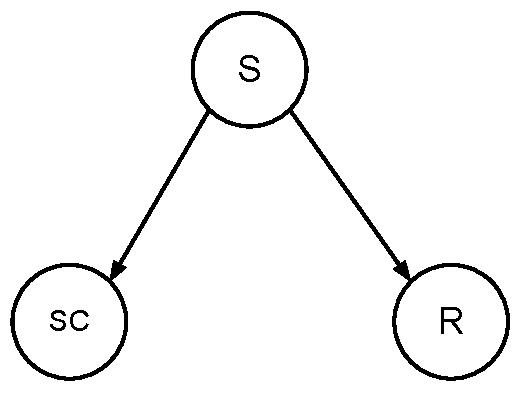
\includegraphics[width=.5\textwidth]{AI-HWK-3_1.pdf}
    \caption{Dynamic Bayesian Network.}\label{fig:3-1}
  \end{figure}

  In this problem S is the hidden variable, R and SC are evidence
  variables, so in order to make only one evidence variable, we can
  combine R and SC into one variable. And the definition of HMM is
  defined by the following elements.  \\
  Initial distribution $P(S_0) = 0.7$. \\ 
  Transitions: $P(S_t|S_{t-1}) = 0.8$ and $P(S_t|\neg
  S_{t-1})=0.3$. \\
  Emissions: $P(R,SC|S) = ,~ P(\neg R,SC|S) = ,~ P(R,\neg SC|S) = ,
  P(\neg R, \neg SC|S) = $
 
}
Formulate this information as a dynamic Bayesian network that the
professor could use to filter or predict from a sequence of
observations. Then reformulate it as a hidden Markov model that has
only a single observation variable. Give the complete probability
tables for the model.

\section{Execise 15.14}
For the DBN specified in Exercise 15.13 and for the evidence values \\
$e_1 =$ not red eyes, not sleeping in class \\
$e_2 =$ red eyes, not sleeping in class \\
$e_3 =$ red eyes, sleeping in class \\
perform the following computations:
\begin{enumerate}[a.]
\item State estimation: Compute $P(EnoughSleep_t|e_{1:t})$ for each
  of $t = 1, 2, 3$.
\solution{
  By applying the Markov property, we get the following result: 
  \begin{align*}
    P(S_0) & = 0.7 \\ 
    P(S_1) & = P(S_1|S_0)P(S_0) + P(S_1|\neg S_0)P(\neg S_0) = 0.65 \\
    P(S_1|e_1) & = \alpha P(e_1|S_1)P(S_1)  = \langle 0.86, 0.136
    \rangle \\
    P(S_2|e_{1:2}) &= \alpha P(e_2|S_2)P(S_2|e_1) = \langle 0.501,
    0.499 \rangle \\ 
    P(S_3|e_{1:2}) = \sum_{S_2}P(S_3|s_2)P(s_2|e_{1:2}) = \langle
    0.55, 0.45 \rangle \\ 
    P(S_3|e_{1:3}) = \alpha P(e_3|S_3)P(S_3|e_{1:2}) = \langle
    0.1045, 0.8955 \rangle 
  \end{align*}
}
\item Smoothing: Compute $P(EnoughSleep_t|e_{1:3})$ for each of $t =
  1,2,3$.
\solution{
  Backward messages can be computed as : \\
  \begin{align*}
    P(e_3|S_3) &= \langle 0.2*0.1, 0.7*0.3 \rangle \\ 
    & = \langle 0.02, 0.21\rangle \\ 
    P(e_3|S_2) &= \sum_{s_3}P(e_3|s_3)P(s_3)P(s_3|S_2) \\
    & = \langle 0.02*0.8+0.21*0.2, 0.02*0.3+0.21*0.7 \rangle \\ 
    & = \langle 0.059, 0.15 \rangle \\
    P(e_{2:3}|S_1) &= \sum_{s_2}P(e_2|s_2)P(e_3|s_2)P(s_2|S_1) \\ 
    & = \langle 0.023 , 0.056 \rangle 
  \end{align*}
  And by combining the backward and forward messages we have: 
  \begin{align*}
    P(S_1|e_{1:3}) & = \alpha P(S_1|e_1)P(e_{2:3}|S_1) \\ 
    & = \langle 0.7277, 0.2723 \rangle \\ 
    P(S_2|e_{1:3}) & = \alpha P(S_2|e_1)P(e_3|S_1) \\ 
    & = \langle 0.2757, 0.7243 \rangle \\
    P(S_3|e_{1:3}) & = \langle 0.1045, 0.895 \rangle \\
  \end{align*}
}
\item Compare the filtered and smoothed probabilities for $t = 1$ and
  $t = 2$.
\solution{
  The smoothed analysis places the time the student started sleeping
  poorly one step earlier than filtered analysis, integrating future
  observations indicating lack of sleep at the last step. 
}
\end{enumerate}

\section{Execise 15.15}
Suppose that a particular student shows up with red eyes and sleeps in
class every day. Given the model described in Exercise 15.13, explain
why the probability that the student had enough sleep the previous
night converges to a fixed point rather than continuing to go down as
we gather more days of evidence. What is the fixed point? Answer this
both numerically (by computation) and analytically.
\solution{
  The probability reaches a fixed point because there is always some
  chance of spontaneously starting to sleep well again, and the
  students who sleep well sometimes have red eyes and sleep in
  class. Even if we knew for sure that the student didn't sleep well
  on day t, and that they slept in class with red eyes on day t+1,
  there would be a chance that the7y slept well on day t+1. 
  So, numerically one can repeatedly apply the forward equations to
  find equilibirum probabilities of $\langle 0.043, 0.957\rangle$. 
  Analytically, we are trying to  find teh vector $(p_0,p_1)^T$, which
  is the fixed point to the forward equation, which one can pose in
  matrix form as 
  \[(p_0,p_1)^T = \alpha \begin{pmatrix} 0.016 & 0.006 \\ 0.042 &
   0.147 \end{pmatrix} (p_0,p_1)^T\]
  where $\alpha$ is a normalization constant. That is, $(p_0,p_1)^T$ is
  an eigenvector of the given matrix. Computing, we find that  the only
  positive eigenvalue is 0.1487, which has eigenvector (normalized to
  sum to one) $(0.0432,0.9568)^T$, just as we numerically computed. 
}
\end{document}
